\documentclass[12pt]{article}
\usepackage[top=1in, bottom=1in, left=1in, right=1in]{geometry}

\usepackage{setspace}
\onehalfspacing

\usepackage{amssymb}
%% The amsthm package provides extended theorem environments
\usepackage{amsthm}
\usepackage{epsfig}
\usepackage{times, paralist}
\renewcommand{\ttdefault}{cmtt}
\usepackage{amsmath}
\usepackage{graphicx} % for graphics files
\usepackage{tabu}

% Draw figures yourself
\usepackage{tikz} 

% writing elements
\usepackage{mhchem}

% The float package HAS to load before hyperref
\usepackage{float} % for psuedocode formatting
\usepackage{xspace}

% from Denovo Methods Manual
\usepackage{mathrsfs}
\usepackage[mathcal]{euscript}
\usepackage{color}
\usepackage{array}

\usepackage[pdftex]{hyperref}
\usepackage[parfill]{parskip}

% math syntax
\newcommand{\nth}{n\ensuremath{^{\text{th}}} }
\newcommand{\ve}[1]{\ensuremath{\mathbf{#1}}}
\newcommand{\Macro}{\ensuremath{\Sigma}}
\newcommand{\rvec}{\ensuremath{\vec{r}}}
\newcommand{\vecr}{\ensuremath{\vec{r}}}
\newcommand{\omvec}{\ensuremath{\hat{\Omega}}}
\newcommand{\vOmega}{\ensuremath{\hat{\Omega}}}
\newcommand{\sigs}{\ensuremath{\Sigma_s(\rvec,E'\rightarrow E,\omvec'\rightarrow\omvec)}}
\newcommand{\el}{\ensuremath{\ell}}
\newcommand{\sigso}{\ensuremath{\Sigma_{s,0}}}
\newcommand{\sigsi}{\ensuremath{\Sigma_{s,1}}}
%---------------------------------------------------------------------------
%---------------------------------------------------------------------------
\begin{document}
\begin{center}
{\bf NE 250, F17\\
November 2, 2017 
}
\end{center}

We've derived the Transport Equation, from it derived the Diffusion Equation, and looked at ways to solve the diffusion equation in both fixed source and multiplying media. We also talked about the TE in the integral form, and looked at the adjoint equation in detail. 

The \textbf{Multigroup Approximation} (from L\&M 2.2)\\
We begin by setting up an energy grid, where $E_0$ is the highest energy value and $E_G$ is the lowest. We get $G-1$ groups and call the group between edge $g$ and edge $g-1$ group $g$. 

\begin{center}
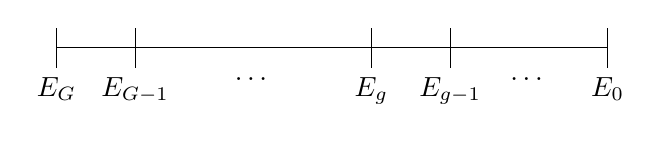
\begin{tikzpicture}
\draw (0,0)--(7,0);
\draw (0,-0.25)--(0, 0.25);
\draw (1,-0.25)--(1, 0.25);
\draw (4,-0.25)--(4, 0.25);
\draw (5,-0.25)--(5, 0.25);
\draw (7,-0.25)--(7, 0.25);
\node[below] at (0,-.25) {$E_G$};
\node[below] at (1,-.25) {$E_{G-1}$};
\node[below] at (2.5,-.25) {$\dots$};
\node[below] at (4,-.25) {$E_g$};
\node[below] at (5,-.25) {$E_{g-1}$};
\node[below] at (6,-.25) {$\dots$};
\node[below] at (7,-.25) {$E_0$};
\end{tikzpicture}
\end{center}

We use this grid to define the group flux
\[
\psi_g(\vecr, \vOmega) \equiv \int_{E_g}^{E_{g-1}} dE\: \psi(\vecr, \vOmega, E)
\]
Note that the continuous $\psi$ is in units of per eV, while the group angular flux is not, it includes all of the neutrons over that energy group. What we want to do next, is derive an equation whose solution is $\psi_g$, which means we will integrate the entire TE over energy. 

To perform that integral, we need to introduce an approximation. The one we will talk about now is \textit{assume the angular flux is separable in energy}:
\[
\psi(\vec{r}, \vOmega, E) \approx f(E)\psi_g(\vec{r}, \vOmega)\:, \quad E_g < E \leq E_{g-1}\:,
\]
where $f(E)$ is normalized such that $\int_g dE\: f(E) = 1$ (note that this means $f$ has units of per eV). We substitute and/or use this in the regular TE and integrate over energy. Here's how that works term by term.
%
\begin{itemize}
\item Streaming:
\[
\int_{E_g}^{E_{g-1}} dE\: \vOmega \cdot \nabla \psi(\vec{r}, \vOmega, E) = \int_{E_g}^{E_{g-1}} dE\: \vOmega \cdot \nabla f(E)\psi_g(\vec{r}, \vOmega) = \vOmega \cdot \nabla \psi_g(\vec{r}, \vOmega)
\]

\item External (distributed fixed) source:
\[q_{g}(\vec{r}, \vOmega) \equiv \int_{E_g}^{E_{g-1}} dE\: q(\vec{r}, \vOmega, E)\]

\item Fission Source:
\begin{align*}
\int_{E_g}^{E_{g-1}} dE\: &\frac{\chi(E)}{4 \pi}\int_0^{\infty} dE' \: \nu(E') \Sigma_f(E') \int_{4 \pi} d\vOmega' \:\psi(\vec{r}, E', \vOmega') \\
&\chi_g \equiv \int_{E_g}^{E_{g-1}} dE\: \chi(E) \\
& \int_{4 \pi} d\vOmega' \:\psi_g(\vec{r}, \vOmega') = \phi_g(\vec{r})\\
& \int_0^{\infty} dE' \: \nu(E') \Sigma_f(E') = \sum_{g'=1}^G \int_{E_g'}^{E_{g'-1}} dE'\: \nu(E') \Sigma_f(E')
\end{align*}
These second two items combine to form the fission source from group $g'$. We also need to define
\[
\nu\Sigma_{fg'} = \int_{E_g'}^{E_{g'-1}} dE'\: \nu(E') \Sigma_f(E') f(E')
\]
and therefore the fission source in group $g$ is
\[
q_{fg} = \frac{\chi_g}{4 \pi}\sum_{g'=1}^G \nu\Sigma_{fg'} \phi_{g'}(\vec{r})
\]

\item Scattering term:
\[
q_{s,gg'}(\vOmega) \equiv \int_{E_g}^{E_{g-1}} dE \int_{E_g'}^{E_{g'-1}} dE' \int_{4 \pi} d\vOmega' \: \Sigma_s(E'\rightarrow E, \vOmega' \cdot \vOmega) \psi(\vec{r}, E', \vOmega')
\]
If we generically define the scattering cross section this we, we can get this general scattering expression
\begin{align*}
\Sigma_{s,gg'}(\vOmega' \cdot \vOmega) & \equiv \int_{E_g}^{E_{g-1}} dE \int_{E_g'}^{E_{g'-1}} dE' \: \Sigma_s(E'\rightarrow E, \vOmega' \cdot \vOmega) f(E')\\
q_{s,g}(\vOmega) &= \sum_{g'=1}^G \int_{4 \pi} d\vOmega' \Sigma_{s,gg'}(\vOmega' \cdot \vOmega) \psi_{g'}(\vec{r}, \vOmega')
\end{align*}

\item Total interaction:
\begin{align*}
\Sigma_{tg}(\vec{r}) &= \int_{E_g}^{E_{g-1}} dE\: \Sigma_t(\vec{r}, E)f(E)\\
\text{term }&= \Sigma_{tg} \psi_g(\vec{r}, \vOmega)
\end{align*}

\end{itemize}
%
We can combine all of this to get a conventional, general expression for the \textbf{multigroup TE}.
\begin{align*}
[\vOmega \cdot \nabla + \Sigma_{tg}(\vec{r})]\psi_g(\vec{r}, \vOmega) =&  \sum_{g'=1}^G \int_{4 \pi} d\vOmega'\: \Sigma_{s,gg'}(\vecr, \vOmega' \cdot \vOmega) \psi_{g'}(\vec{r}, \vOmega')\\
&+\frac{\chi_g}{4 \pi}\sum_{g'=1}^G \nu\Sigma_{fg'}(\vec{r}) \phi_{g'}(\vec{r}) + q_g(\vec{r}, \vOmega)
\end{align*}
If we want, we can integrate this equation over angle to get a balance equation and from there derive the multigroup diffusion equation.

---------------------------------\\
\textbf{Group Constants}\\
To solve this equation, we need all of the collapsed cross section values to come from somewhere (for this to be accurate, we need the detailed energy dependence of the cross sections and the spectral weighting function, $f(E)$, to be known). 

For smoothly varying parts of the cross section, it is reasonably easy to make weighting function assumptions. However, in resonance regions even very fine group structures are insufficient and we get self-shielding effects that will be missed. There are a variety of methods to attempt to capture this behavior, but we will not go into them here.

In a general sense, we often 
\begin{enumerate}
\item start with ENDF data (1000s of energy groups), and then do an infinite medium or 1-D transport calculation and use the results to collapse the data to 100s of energy groups.

\item Following this we often do another transport calculation at the level of a unit cell or assembly and then collapse in energy and homogenize in space, getting us few to 10s of groups.\\
We will take, e.g.\ an assembly from the middle of the core and put reflecting boundary conditions on all sides and solve for either $\psi_g(\vec{r}, \vOmega)$ or $\phi_{l,g}^m(\vec{r})$ (see below) to use in the collapsing.

\item Finally, we do a core level calculation with diffusion theory. 
\end{enumerate}

Collapsing in energy with fine groups (indexed $j$) into coarse group (indexed $h$):
\[
\Sigma_{h} \equiv \frac{\sum_{j \in h} \Sigma_{j} \phi_j(\vec{r})}{\sum_{j\in h} \phi_j(\vec{r})}
\]
and you would replace $\phi_g$ with $\psi_g$ or $\phi_{l,g}^m$ if doing scattering. 

Homogenizing in space (flux-weighting):
\[
\Sigma_j^{homog} \equiv \frac{\int_V dV \: \Sigma_j(\vec{r}) \phi_g(\vec{r})}{\int_V dV \: 
\phi_g(\vec{r})}
\]
where $V$ is a region made up of different nuclides at each point. 

-----------------------------

Discuss structure of iterations.


----------------------------------------------\\
\textbf{Alternative Derivation} 

(Please note: the deep nature of this discussion is oriented for those who really are interested in this topic)

We can remove the requirement of separability in energy, which allows us to define better multigroup constants (we don't need the energy weighting function). \\
To facilitate this, we can use the \textit{Legendre expansion technique} as we did before, which allows for better weighting of the multigroup cross sections.

Recall the Legendre addition theorem and flux moment definition:
\begin{align*}
P_l(\vOmega' \cdot \vOmega) &= \frac{1}{2l+1}\sum_{m=-l}^l Y^*_{lm}(\vOmega)Y_{lm}(\vOmega')\\
\phi_{l}^{m}(\vec{r},E') &= \int_{4 \pi} d\vOmega'\: Y_{lm}(\vOmega') \psi(\vec{r}, \vOmega', E') \\
\psi(\vec{r}, \vOmega', E') &= \sum_{l=0}^{\infty} \sum_{m=-l}^l Y^*_{lm}(\vOmega)\phi_{l}^{m}(\vec{r},E')\\
\Sigma_s(E'\rightarrow E, \vOmega' \cdot \vOmega) &= \sum_{l=0}^{\infty} (2l+1) \Sigma_{s,l}(E'\rightarrow E) P_l(\vOmega' \cdot \vOmega)
\end{align*}
We will apply this in our TE 
%
\begin{align*}
\bigl[\vOmega \cdot \nabla + \Sigma_t\bigr] \psi(\vec{r}, E, \vOmega) &= \frac{\chi(E)}{4 \pi}\int_0^{\infty} dE' \: \nu(E') \Sigma_f(E') \int_{4 \pi} d\vOmega' \:\psi(\vec{r}, E', \vOmega') + q(\vec{r}, E, \vOmega)\\
 &+\sum_{l=0}^{\infty} \sum_{m=-l}^l Y^*_{lm}(\vOmega)\int_0^{\infty} dE' \Sigma_{s,l}(E'\rightarrow E) \phi_{l}^{m}(\vec{r},E')
\end{align*}
%
and integrate over energy to get groups (note that we don't change anything compared to before with the streaming term or the external source).
%
\begin{itemize}
\item Scattering:\\
We can rewrite the scattering source term
\[
q_{s,gg'} = \sum_{l=0}^{\infty} \sum_{m=-l}^l Y^*_{lm}(\vOmega)\int_{E_g}^{E_{g-1}} dE \int_{E_g'}^{E_{g'-1}} dE' \: \Sigma_{s,l}(E'\rightarrow E)\phi_{l}^{m}(\vec{r},E')
\]
We can use the angular flux moments to define a group scattering cross section moment:
\[
\Sigma_{sl,gg'} \approx \dfrac{\int_{E_g}^{E_{g-1}} dE \int_{E_g'}^{E_{g'-1}} dE' \: \Sigma_{s,l}(E'\rightarrow E)\phi_{l}^{m}(\vec{r},E')}{\phi_{l,g'}^{m}(\vec{r})}
\]
Finally
\begin{align*}
q_{s,gg'} &= \sum_{l=0}^{\infty} \sum_{m=-l}^l Y^*_{lm}(\vOmega)\Sigma_{sl,gg'}\phi_{l,g'}^{m}(\vec{r})\\
q_{s,g} &= \sum_{l=0}^{\infty} \sum_{m=-l}^l Y^*_{lm}(\vOmega)\sum_{g'=1}^G \Sigma_{sl,gg'}\phi_{l,g'}^{m}(\vec{r})
\end{align*}

\item Total interaction:\\
Our first thought is to define the group total cross section this way
\[
\Sigma_{tg}(\vec{r}, \vOmega) = \dfrac{\int_{E_g}^{E_{g-1}} dE\: \Sigma_t(\vec{r}, E) \psi(\vec{r}, \vOmega, E)}{\psi_g(\vec{r}, \vOmega)}
\]
but this adds angular dependence to the total cross section, and most codes and data aren't set up to handle this. \\
Instead, We can use the Legendre expansion of the flux and define total cross section moments as well.
\[
\int_{E_g}^{E_{g-1}} dE\: \Sigma_t(\vec{r}, E)\sum_{l=0}^{\infty} \sum_{m=-l}^l Y^*_{lm}(\vOmega)\phi_{l}^{m}(\vec{r},E) = \sum_{l=0}^{\infty} \sum_{m=-l}^l Y^*_{lm}(\vOmega)\int_{E_g}^{E_{g-1}} dE\: \Sigma_{t}(\vec{r},E)\phi_{l}^{m}(\vec{r},E)
\]
Thus, we define a total cross section moment:
\[
\Sigma_{tl,g}(\vec{r}) = \dfrac{\int_{E_g}^{E_{g-1}} dE\: \Sigma_t(\vec{r}, E) \phi_l^m(\vec{r}, E)}{\phi_{l,g}^m(\vec{r})}
\]
and the whole term becomes
\[
= \sum_{l=0}^{\infty} \sum_{m=-l}^l Y^*_{lm}(\vOmega)\Sigma_{tl,g}(\vec{r})\phi_{l,g}^{m}(\vec{r})
\]

\item Fission remains pretty easy since it already only requires the scalar flux. 
\[
\nu\Sigma_{fg'} = \dfrac{\int_{E_g'}^{E_{g'-1}} dE'\: \nu(E') \Sigma_f(E')\phi(\vec{r}, E')}{\phi_{g'}(\vec{r})}
\]
\end{itemize}

We can combine all of this, and we add another $\Sigma_g \psi_g$ to both sides:
\begin{align*}
[\vOmega \cdot \nabla &+ \Sigma_{tg}(\vec{r})]\psi_g(\vec{r}, \vOmega) =  \frac{\chi_g}{4 \pi}\sum_{g'=1}^G \nu\Sigma_{fg'}(\vec{r}) \phi_{g'}(\vec{r}) + q_g(\vec{r}, \vOmega)\\
&+ \sum_{l=0}^{\infty} \sum_{m=-l}^l Y^*_{lm}(\vOmega)\sum_{g'=1}^G \bigl[\Sigma_{sl,gg'} + \bigl(\underbrace{\Sigma_{tg}(\vec{r})}_{\text{balances rhs}} - \Sigma_{tl,g}(\vec{r}) \bigr) \delta_{gg'}  \bigr]\phi_{l,g'}^{m}(\vec{r})
\end{align*}
%
This form looks just like the first version we derived, but the scattering term is a little wonky. \\
Note that we still have a problem. We added the $\Sigma_{tg}(\vec{r})$ to make the equation look right, but haven't explained what it is. \\
If we just weight it with the scalar flux ($P_0$ version), we get
\[
\Sigma_{tg}(\vec{r}) = \Sigma_{tg,0}(\vec{r}) = \dfrac{\int_{E_g}^{E_{g-1}} dE\:\Sigma_{t}(\vec{r}, E) \phi(\vec{r}, E)}{\phi_g(\vec{r})}
\]
This is called the ``consistent $P_N$ approximation". 

A more elegant technique uses the observation that for scattering, we usually truncate the expansion at some $l=L$. \\
We can then choose $\Sigma_{tg}(\vec{r})$ to make the $l=L+1$th component to be small. That is
\[
\sum_{m=-(L+1)}^{L+1} Y^*_{(L+1)m}(\vOmega)\sum_{g'=1}^G \bigl[\Sigma_{s(L+1),gg'} + \bigl(\Sigma_{tg}(\vec{r}) - \Sigma_{t(L+1),g}(\vec{r}) \bigr) \delta_{gg'}  \bigr]\phi_{(L+1),g'}^{m}(\vec{r}) \approx 0\:.
\]
For reactors, it is usually the case that scattering into a given group is equal to scattering out of it for most energy groups (which ones wouldn't this be true for?).\\
We can then say
\begin{align*}
\sum_{g'=1}^G \Sigma_{s(L+1),gg'}\phi_{(L+1),g'}^{m}(\vec{r}) &\approx \sum_{g'=1}^G \Sigma_{s(L+1),g'g}\phi_{(L+1),g'}^{m}(\vec{r})\\
\Sigma_{tg}(\vec{r}) &= \Sigma_{t(L+1),g}(\vec{r}) - \sum_{g'=1}^G \Sigma_{s(L+1),g'g}
\end{align*}
%
This definition is called the ``extended transport approximation".



\subsection*{Nuclear Data}
Nuclear data, to me, is always most viscerally connected to discussions about energy and multigroup. This isn't really true, but energy dependence and the variation of nuclear data with energy for neutron interactions with isotopes we care about is most of what makes nuclear computation hard. Hence, now is the time I'd like to talk about nuclear data. 

We need a description of all of the physical interactions happening inside a nuclear reactor that we can use in our equation. An \textit{evaluated nuclear data file} is a collection of various data enabling to reconstruct, for each isotope, its cross-section's 
\begin{compactitem}
\item general information
\item resonance parameters 
\item angular distribution for emitted particles 
\item energy distribution for emitted particles 
\item energy-angle distribution for emitted particles 
\item thermal neutron scattering law data 
\item radioactivity and fission-product yield data 
\item multiplicities for radioactive nuclide production 
\item cross-sections for radioactive nuclide production
\end{compactitem}

There are many evaluations coming from various countries such as: USA, Europe, Japan, Russia, China, \dots Getting from experimental data (what we have of it) + theory (however accurate that is) to data that can actually be used in a code is no small feat. And, that process is sort of a mess...
\begin{figure}[h!]
    \begin{center}
    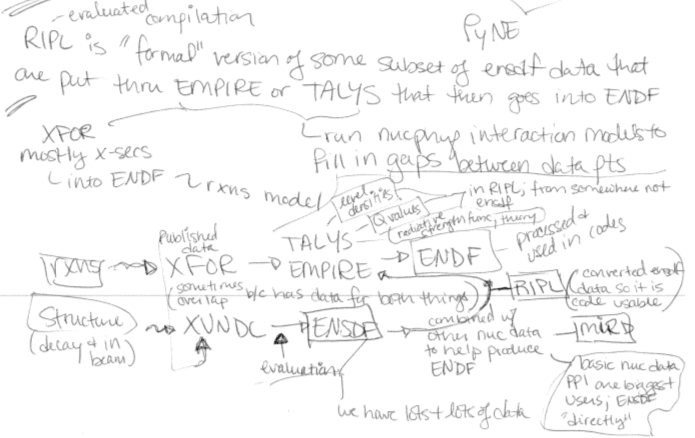
\includegraphics[keepaspectratio, width = 6 in]{../figs/data-notes}
    \end{center}
    \caption{Notes from a meeting where someone tried to explain this to me}
    \label{fig:datanotes}
\end{figure}
\begin{figure}[h!]
    \begin{center}
    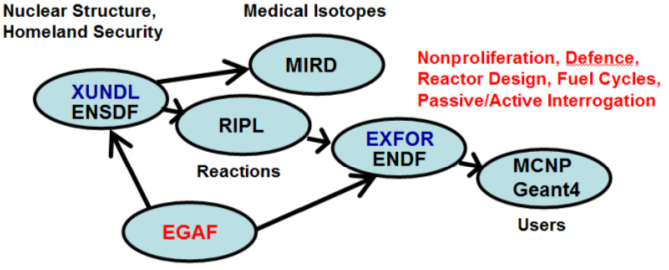
\includegraphics[keepaspectratio, width = 4.5 in]{../figs/hurst-code-map}
    \end{center}
    \caption{A more coherent (but less comprehensive) set}
    \label{fig:hurstfig}
\end{figure}

We won't go through all of this, but I think it's important to have context about what this is and how confusing it can be. There is a lot of data and many formats. In computation you will pretty much only need to interface with ENDF and its equivalents. 

The data that we use is complicated, and can be quite different depending on the application we're interested in. Let's look at some (back to ppt).

%-------------------------------------------------------------
%-------------------------------------------------------------
\subsection*{Physics Impacts}
We are often able to use knowledge about the physics to inform method development or, at the very least, choose which methods are more appropriate given our physics. 

For example, you may notice is how, in particular, Fast and Thermal reactor physics differ. We often need different codes to deal with LWRs and FRs (note: CASL and NEAMS are different initiatives...). 
%
Many of the assumptions employed in traditional LWR methods do not apply:
\begin{compactitem}
\item Lack of a 1/E energy spectrum as a basis for the calculation of resonance absorption.
\item Upscattering resulting from the thermal motion of the scattering nuclei may be neglected.
\item Inelastic, (n, 2n), and anisotropic scattering are quite important.
\item Long mean free paths imply global coupling. That is, local reactivity effects impact the entire core.  
\item The energy range where neutrons induce fission and the energy range where the fission neutrons appear strongly overlap.
\end{compactitem}
%
Other physics considerations have high priority in FR methods
\begin{compactitem}
\item Detailed energy modeling for resonance structure (core/reflector).
\item Transport and anisotropy effects are more important at high energy.
\end{compactitem}
%
In general, a distinct set of physics analysis and core design tools with tailer assumptions have been and are being developed for FR analysis.




\end{document}
